\documentclass[acmtog]{acmart}
\usepackage{graphicx}
\usepackage{subfigure}
\usepackage{natbib}
\usepackage{listings}
\usepackage{bm}
\usepackage{amsmath}

\definecolor{blve}{rgb}{0.3372549 , 0.61176471, 0.83921569}
\definecolor{gr33n}{rgb}{0.29019608, 0.7372549, 0.64705882}
\makeatletter
\lst@InstallKeywords k{class}{classstyle}\slshape{classstyle}{}ld
\makeatother
\lstset{language=C++,
	basicstyle=\ttfamily,
	keywordstyle=\color{blve}\ttfamily,
	stringstyle=\color{red}\ttfamily,
	commentstyle=\color{magenta}\ttfamily,
	morecomment=[l][\color{magenta}]{\#},
	classstyle = \bfseries\color{gr33n}, 
	tabsize=2
}
\lstset{basicstyle=\ttfamily}
% Title portion
\title{Assignment 2:\\ {Assignment 2 : Geometric Modeling}} 
\author{Name:\quad Yin Hairui  \\ student number:\ 2020533028
\\email:\quad yinhr@shanghaitech.edu.cn}

% Document starts
\begin{document}
\maketitle

\vspace*{2 ex}

\section{Introduction}
The followings are all jobs that have been doen, containing basic task and the bonus of NURBS surface!
\begin{itemize}
\item implementation of basic iterative de Casteljau Bézier vertex evaluation
\item  Construction of Bézier Surface with normal evaluation
\item Rendering a Bézier Surface
\item Generate tea object
\item Finish NURBS surface construction
\end{itemize}
\section{Implementation Details}
\subsection{iterative de Casteljau Algorithm}
First we need to finish the part in "bezier.cpp" of "Vertex BezierCurve::evaluate". The main idea of the realization comes from a iterative equation:
$$P_{i,j}=(1-u)P_{i-1,j}+uP_{i-1,j+1}$$
where $i=1,2,...,n,j=0,1,...,n-i$
\newline
I define a assistant function called deCasteljau() outside evaluate() to help iterative loops.
\subsection{Construction of Bézier Surface}
The main idea of create a surface is to firstly, construct m intermediate Bézier curves based on the corresponding n control points and evaluate m points at parameter v, and then, construct another Bézier curve based on the m points and evaluate the point at u.\\
In the process, we can find one vertex with position and its tangent in u direction. Since Bézier Surface is a sum of vertices weights, the position is ensured.\\
However, to find the normal of the point in surface, we have to repeat evaluate process in another diretion. With the result two vertices, do glm::cross() to find the normal.\\
The result is a Vertex.
\subsection{Rendering a Bézier Surface}
The target of this mission is to store vertex information into the class Object, load VAO, VBO and EBO, and use member function to draw corresponding graph.\\
I modify the function parameters in Object::initialize() to pass necessary vertices and indices to build VAO, VBO and EBO. The vertices is in vector<Vertex> form and indices is a index vertex.\\
After finishing these basic function, I define a self made $3\times3$ control points in main.cpp, and use Bézier Surface function to generate sample points. Then after dealing with the data, I pass vertices and indices into Object to draw my Bézier Surface.\\
The shader used is called easyshader, with color of $vec4(1.0f,1.0f,1.0f,1.0f)$.
\subsection{Generate tea object}
The tea object is stored in "assets/tea.bzs". With the surface number, vertex number and range of the surface, we can load it into vectors and create the corresponding vertices vector and indices vector. Since the data is continuous (different surface share the same edge), it ensures L0-th order continuity.\\
After generating data, we can load it into Object and draw the graph in the screen, with the same procedure as previous mission.
\subsection{NURBS surface}
de Boor algorithm also works for NURBS surface, with a little adjustment. NURBS requires one more dimension, which is the weight of control points, ranging from $[0,1]$. In the code, I create a new deBoor function with parameters in vec4 and return value in vec4. The new control point sending into the function is $(x\times w, y\times w, z\times w, w)$, and we should divide the weight after deBoor result to transform it back to 3D.\\
To see the effect of NURBS clearly, I use the same data as surface part, with some adjustments in weight of particular points.
To render the normal control point, we can set weight to $1$ for every point.

\section{Results}
The results are pictures following.\\
As we can see, there is only a point in SURBS changed its weight to $0.1$ and that causes a big difference in the curve that point controls.\\
\begin{figure}[h]
	\centering
	\subfigure[Left]
	{
		\begin{minipage}[b]{.4\linewidth}
			\centering
			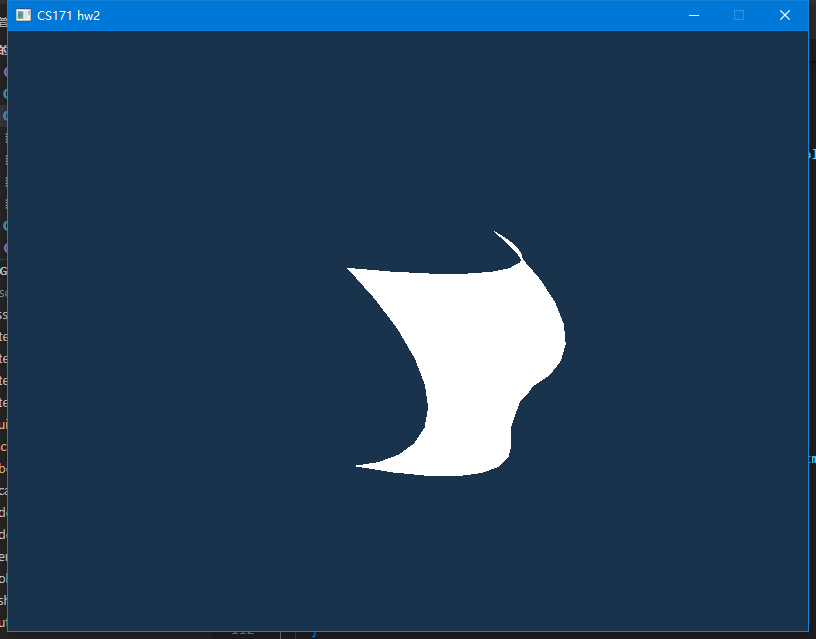
\includegraphics[scale=0.108]{surface_left.png}
		\end{minipage}
	}
	\subfigure[Left]
	{
		\begin{minipage}[b]{.4\linewidth}
			\centering
			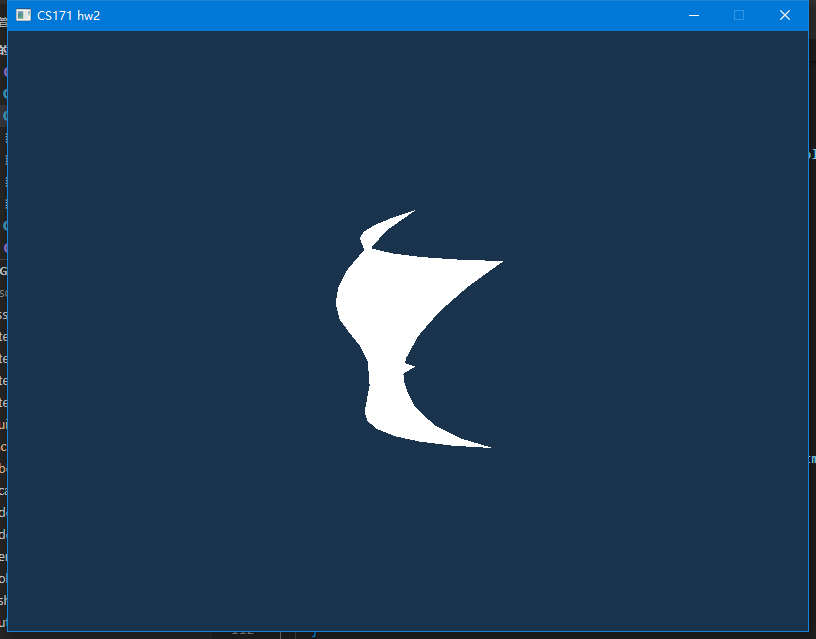
\includegraphics[scale=0.106]{surface_right.png}
		\end{minipage}
	}
	\caption{Bézier Surface}
\end{figure}
\begin{figure}[h]
	\centering
	\subfigure[Bottom]
	{
		\begin{minipage}[b]{.4\linewidth}
			\centering
			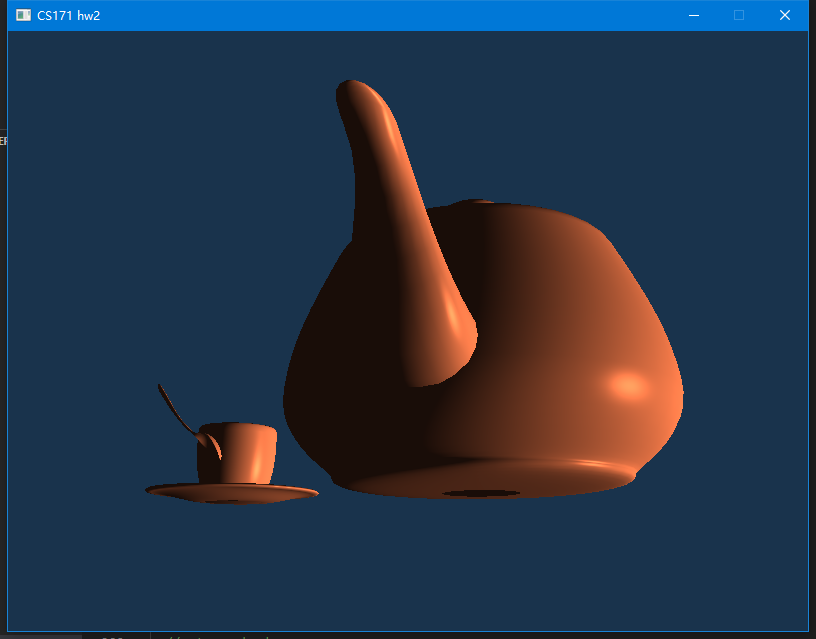
\includegraphics[scale=0.108]{tea_bottom.png}
		\end{minipage}
	}
	\subfigure[Head]
	{
		\begin{minipage}[b]{.4\linewidth}
			\centering
			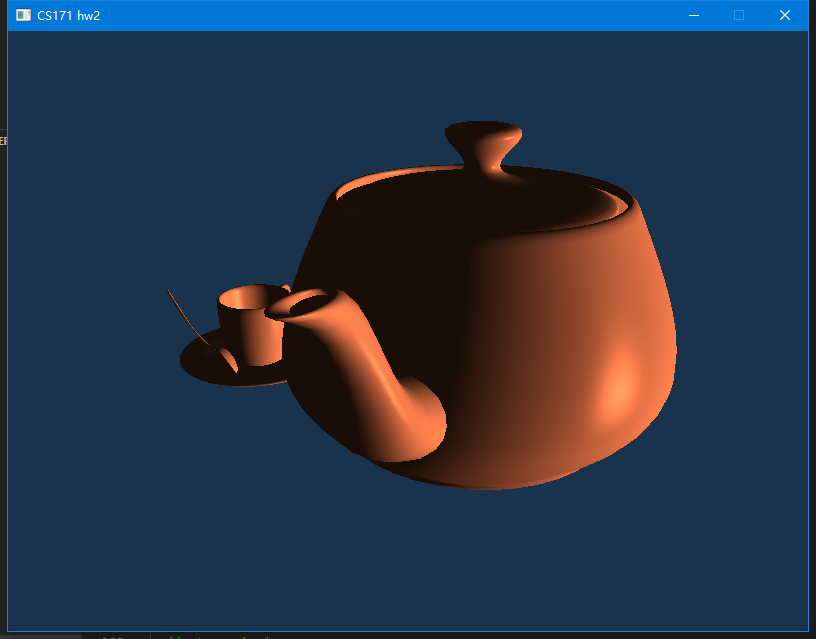
\includegraphics[scale=0.106]{tea_head.png}
		\end{minipage}
	}
	\caption{Teapot and spone}
\end{figure}
\begin{figure}[h]
	\centering
	\subfigure[Original Surface]
	{
		\begin{minipage}[b]{.4\linewidth}
			\centering
			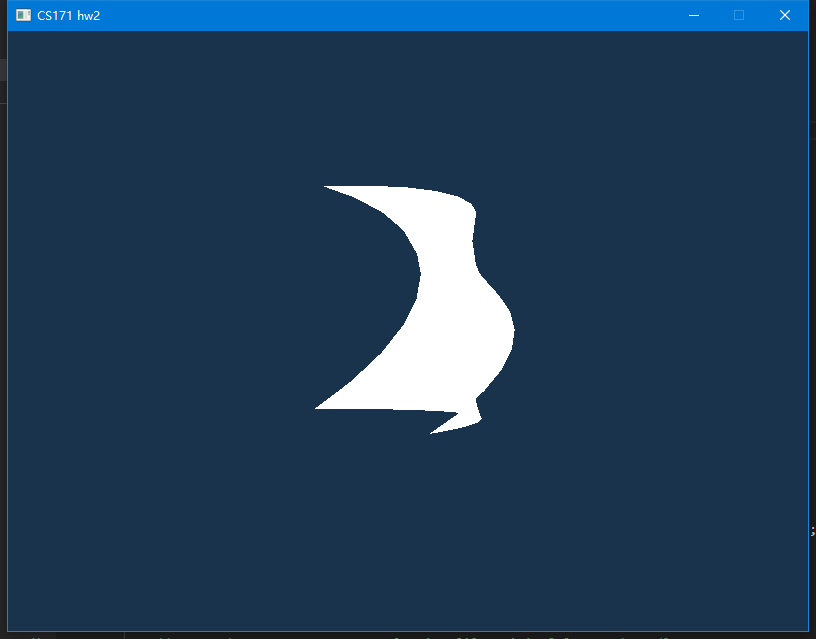
\includegraphics[scale=0.108]{original.png}
		\end{minipage}
	}
	\subfigure[Changed weight surface]
	{
		\begin{minipage}[b]{.4\linewidth}
			\centering
			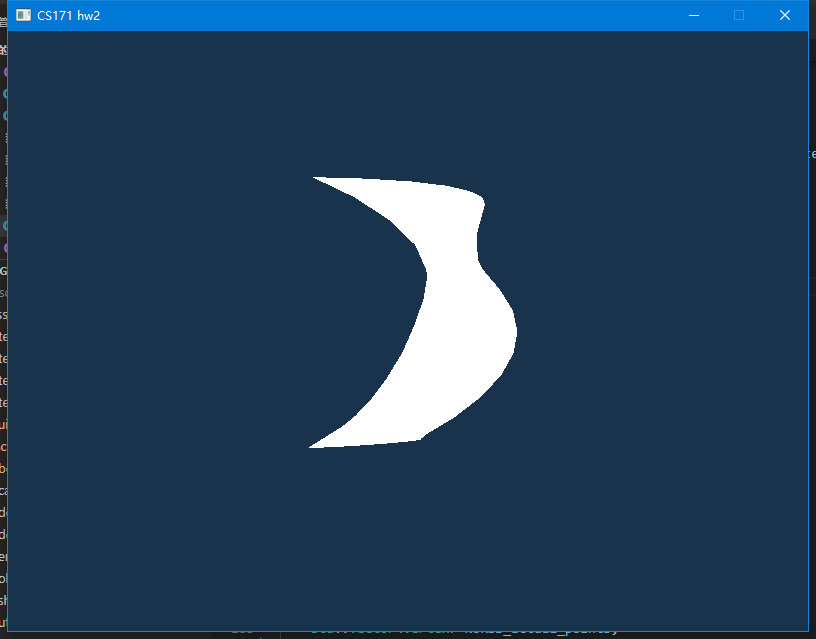
\includegraphics[scale=0.106]{chenged_weight.png}
		\end{minipage}
	}
	\caption{NURBS}
\end{figure}
\end{document}
